% =============================================================================
\bloco{1}{Consumption, present bias and interest rates}{Kurlat chs.~6, 9; Romer ch.~8 \,\textbullet\, 25 points}

\questao{(10 points) Objective items.}

\textbf{a)} (3 points) A household lives $T+1$ periods ($t=0,\dots,T$; $T\ge1$) with $u(c)=c^{1-\sigma}/(1-\sigma)$, $\sigma>0$
($\ln c$ if $\sigma=1$), discount factor $0<\beta<1$ and a constant real rate $r>0$; its total wealth (financial plus human,
in present value at $t=0$) is $W$. The share $c_0/W$ is:
\begin{alternativas}
\item $(1-\gamma)/(1-\gamma^{T+1})$ with $\gamma=\beta^{\sigma}(1+r)^{\sigma-1}$
\item $(1-\gamma)/(1-\gamma^{T+1})$ with $\gamma=\beta^{1/\sigma}(1+r)^{1/\sigma-1}$
\item $(1-\gamma)/(1-\gamma^{T+1})$ with $\gamma=\beta$
\item $(1-\gamma)/(1-\gamma^{T+1})$ with $\gamma=[\beta(1+r)]^{\sigma}$
\end{alternativas}
\gabarito{B}
\begin{sol}
\passo{path and budget}{The Euler equation (6.3.9), $c_t^{-\sigma}=\beta(1+r)c_{t+1}^{-\sigma}$, gives $c_t=[\beta(1+r)]^{t/\sigma}c_0$. Leaving assets after $T$ is
wasteful, so (6.3.6) binds: $\sum_{t=0}^{T}c_t(1+r)^{-t}=c_0\sum_{t=0}^{T}\gamma^t=W$ with $\gamma\equiv\beta^{1/\sigma}(1+r)^{1/\sigma-1}$. Summing the geometric
series, $c_0/W=(1-\gamma)/(1-\gamma^{T+1})$ ($1/(T+1)$ as $\gamma\to1$). Mistakes: A takes $\sigma$ for the intertemporal elasticity $1/\sigma$;
C is the log case, right only if $\sigma=1$ or $\beta(1+r)=1$; D makes two mistakes: it takes $\sigma$ for $1/\sigma$ and does not discount
consumption growth in the budget.}
\refbib{Kurlat (2020), ch.~6, \S6.3, eqs.\ (6.3.6) and (6.3.9).}
\end{sol}

\medskip
\textbf{b)} (3 points) \emph{Consumption $\times$ general equilibrium.} A two-period endowment economy with a representative
household: endowments $y_1>0$ and $y_2=(1+g)y_1$, $g>0$; preferences $u(c_1)+\beta u(c_2)$, CRRA with $\sigma>0$, $0<\beta<1$; a bond
in zero net supply pays $r$. The equilibrium real interest rate is:
\begin{alternativas}
\item $r=(1+g)/\beta-1$
\item $r=1/\beta-1$
\item $r=(1+g)^{1/\sigma}-1$
\item $r=(1+g)^{\sigma}/\beta-1$
\end{alternativas}
\gabarito{D}
\begin{sol}
\passo{clearing and price}{A representative household holds none of a bond in zero net supply, so $c_t=y_t$. The Euler
equation (9.1.8), $c_1^{-\sigma}=\beta(1+r)c_2^{-\sigma}$, then gives $1+r=(y_2/y_1)^{\sigma}/\beta=(1+g)^{\sigma}/\beta$: the rate makes the household content
with its growing endowment. Mistakes: A is the log case (right only if $\sigma=1$); B drops growth (right only if $g=0$);
C makes two mistakes: it takes $\sigma$ for the elasticity $1/\sigma$ and drops the discount factor (as if $\beta=1$).}
\refbib{Kurlat (2020), ch.~9, \S9.1, eq.\ (9.1.8), with endowments in place of production.}
\end{sol}

\medskip
\textbf{c)} (2 points, T or F) \emph{Consumption $\times$ credit markets.} Two periods, endowments $(y_1,y_2)$, utility $u(c_1)+\beta u(c_2)$ with
$u$ strictly increasing and strictly concave; the household saves at $r_s$ and borrows at $r_b>r_s$. At the current rates it neither borrows nor
lends, and the first unit saved would strictly lower its utility at the margin. Then any rise in $r_s$, however small,
makes it save.
\gabarito{F}
\begin{sol}
\passo{kink}{Let $m\equiv u'(y_1)/[\beta u'(y_2)]$. Saving $a\ge0$ yields $f(a)=u(y_1-a)+\beta u(y_2+(1+r_s)a)$, strictly concave, with
$f'(0)=\beta u'(y_2)(1+r_s-m)$; the premise is $f'(0)<0$, i.e.\ $m>1+r_s$. At a new rate $r_s'$ with $1+r_s'<m$, still $f'(0)<0$, so $f'(a)<0$
for all $a\ge0$, and borrowing does not involve $r_s$: the household stays put. Only rises beyond $m-(1+r_s)$ make it save.}
\refbib{Kurlat (2020), ch.~6, \S6.2 and Exercise 6.6 (a tax on savings kinks the budget set).}
\end{sol}

\medskip
\textbf{d)} (2 points, T or F) \emph{Consumption $\times$ fiscal policy.} Two periods, utility $u(c_1)+\beta u(c_2)$ with $u$ strictly increasing
and strictly concave, income $y_t$, lump-sum taxes $\tau_t$; the household's saving faces the limit $a\ge-b$, $b\ge0$, which binds. A tax cut
$\Delta>0$ today is financed by a tax increase $(1+r)\Delta$ next period. Then current consumption rises by exactly $\Delta$, for every $\Delta>0$.
\gabarito{F}
\begin{sol}
\passo{threshold}{After the cut $c_2=(1+r)(W-c_1)$ with $W\equiv y_1-\tau_1+\frac{y_2-\tau_2}{1+r}$: the budget line does not move, so the strictly concave
$u(c_1)+\beta u((1+r)(W-c_1))$ has a maximizer $c_1^u$ free of $\Delta$. Only the limit moves, $c_1\le y_1-\tau_1+b+\Delta$, so
$c_1=\min\{c_1^u,\,y_1-\tau_1+b+\Delta\}$. The limit binds before the cut: $\bar\Delta\equiv c_1^u-(y_1-\tau_1+b)>0$, and
$\Delta c_1=\min\{\Delta,\bar\Delta\}$: \textbf{False} for every $\Delta>\bar\Delta$, whatever $u$ and $\beta$.}
\passo{reading}{Up to $\bar\Delta$ the cut is the loan the household could not get, spent one for one; a larger cut makes the limit
slack, and the household saves the rest to pay the later tax (Ricardian equivalence at the margin).}
\refbib{Kurlat (2020), ch.~6, \S6.2 and Exercise 6.5(e).}
\end{sol}

% -----------------------------------------------------------------------------
\questao{(15 points) Discursive. \emph{Consumption $\times$ behavioral economics $\times$ general equilibrium.} Three periods
$t=0,1,2$; in (a)--(c) the real interest rate is zero and the household has wealth $W>0$ at date 0. The self at date $t$
maximizes $u(c_t)+\beta\sum_{s>t}u(c_s)$ with $u(c)=c^{1-\sigma}/(1-\sigma)$, $\sigma>0$ ($\ln c$ if $\sigma=1$), and $0<\beta<1$.}

\textbf{a)} (3 points) Find the plan chosen with commitment (self 0 chooses all three consumptions), by a naive self 0
(who believes future selves will follow its plan) and by a sophisticated self 0 (who anticipates self 1's choice).
In what sense are these preferences time-inconsistent?
\resolespaco
\begin{sol}
\passo{self 1}{With $W_1=W-c_0$, self 1 solves $\max u(c_1)+\beta u(c_2)$ s.t.\ $c_1+c_2=W_1$. The FOC $c_1^{-\sigma}=\beta c_2^{-\sigma}$ gives $c_2=\omega c_1$ with
$\omega\equiv\beta^{1/\sigma}\in(0,1)$, so $c_1=kW_1$ and $c_2=(1-k)W_1$, $k\equiv1/(1+\omega)\in(\frac12,1)$.}
\passo{commitment and naivete}{Under $c_0+c_1+c_2=W$, self 0's FOCs $u'(c_1)=u'(c_2)$, $u'(c_0)=\beta u'(c_1)$ give $c_1=c_2=\omega c_0$:
$(c_0^C,c_1^C,c_2^C)=\frac{W}{1+2\omega}(1,\omega,\omega)$. The naive self 0 expects this plan, so $c_0^N=c_0^C$, and self 1 splits $W_1=\frac{2\omega W}{1+2\omega}$:
$(c_1^N,c_2^N)=\frac{2\omega W}{(1+2\omega)(1+\omega)}(1,\omega)$.}
\passo{sophistication}{By homogeneity, $u(sW_1)=s^{1-\sigma}u(W_1)$, so self 1's rule leaves self 0 the continuation $\beta A(k)u(W_1)$, with
$A(s)\equiv s^{1-\sigma}+(1-s)^{1-\sigma}$ (under log, $A\equiv2$ up to a constant). The FOC of the strictly concave $\max_{c_0}u(c_0)+\beta A(k)u(W-c_0)$
is $c_0^{-\sigma}=\beta A(k)(W-c_0)^{-\sigma}$; with $k=\frac1{1+\omega}$, $1-k=\frac{\omega}{1+\omega}$ and $\omega^{\sigma}=\beta$,
\[c_0^S=\frac{W}{1+\Lambda},\qquad\Lambda\equiv[\beta A(k)]^{1/\sigma}=(1+\omega)^{1-1/\sigma}(\beta+\omega)^{1/\sigma},\qquad
(c_1^S,c_2^S)=\frac{\Lambda W}{(1+\Lambda)(1+\omega)}(1,\omega).\]
Under log, $\Lambda=2\beta$: the sophisticated plan is the naive one.}
\intuicao{$c_1^N/c_1^C=\frac{2}{1+\omega}>1>\frac{2\omega}{1+\omega}=c_2^N/c_2^C$: with nothing new learned, self 1 overturns the plan, since the
weight of $c_2$ relative to $c_1$ is $1$ seen from date 0 and $\beta$ seen from date 1.}
\refbib{Romer (2012), ch.~8, \S8.6 (time-inconsistent preferences) and Problem 8.15; Kurlat (2020), ch.~6, \S6.4.}
\rubrica{
\item Self 1's rule 0.5; commitment 0.5; naive 0.5; sophisticated (continuation, FOC, plan) 1; inconsistency 0.5.
\item Log case solved in place of general $\sigma$: max.\ half. Plans quoted (e.g.\ from Romer 8.15), not derived: max.\ a third.
}
\end{sol}

\textbf{b)} (3 points) Determine when the sophisticated self 0 consumes more, less or the same as the naive one, and
explain the mechanism.
\resolespaco
\begin{sol}
\passo{reduction}{From (a), $c_0^S\lesseqgtr c_0^N\iff\Lambda\gtreqless2\omega\iff\beta A(k)\gtreqless(2\omega)^{\sigma}=\beta2^{\sigma}\iff A(k)\gtreqless A(\tfrac12)$, as $A(\frac12)=2\cdot2^{\sigma-1}=2^{\sigma}$.}
\passo{Jensen}{$A(k)=\varphi(k)+\varphi(1-k)$ with $\varphi(z)=z^{1-\sigma}$, $\varphi''(z)=\sigma(\sigma-1)z^{-\sigma-1}$, and $k\ne\frac12$ (as $\omega<1$) with midpoint $\frac12$.
Strict Jensen: $\sigma>1$ ($\varphi$ convex) $\Rightarrow A(k)>A(\frac12)\Rightarrow c_0^S<c_0^N$; $\sigma<1$ ($\varphi$ concave) $\Rightarrow c_0^S>c_0^N$; $\sigma=1$ ($A\equiv2$) $\Rightarrow c_0^S=c_0^N$.}
\intuicao{Let $R\equiv[A(k)/A(\frac12)]^{1/(1-\sigma)}$, so $A(k)=A(\frac12)R^{1-\sigma}$: the sophisticate's FOC is a naive self's FOC with a gross
return $R<1$ on saving (in both cases above). A lower return raises saving iff the income effect dominates ($\sigma>1$)
and lowers it iff the substitution effect does ($\sigma<1$); under log they cancel and the split drops out.}
\refbib{Romer (2012), Problem 8.15(b)(ii) and ch.~8, \S8.4; Kurlat (2020), Exercise 6.1(e).}
\rubrica{
\item Reduction to $A(k)$ versus $A(\frac12)$ 1 pt; Jensen, three cases 1 pt; mechanism (effective return) 1 pt.
\item Ordering asserted without the convexity argument: 0 for that line. Only the log case treated: max.\ half.
}
\end{sol}

\textbf{c)} (3 points) At date 0 self 0 can buy an illiquid account that locks in the $(c_1,c_2)$ it chooses. What share $x$
of $W$ would a sophisticated self 0 pay for it at most? Show whether $x$ depends on $W$, bound it, give it under log
utility and find how it behaves as $\beta\to1$. What would a naive self 0 pay?
\resolespaco
\begin{sol}
\passo{values}{For weights $w_j>0$, $\max\sum_jw_ju(c_j)$ s.t.\ $\sum_jc_j=W$ has FOCs $w_jc_j^{-\sigma}=\lambda$, so $c_j=Ww_j^{1/\sigma}/S$, $S\equiv\sum_jw_j^{1/\sigma}$, and value
$\frac{W^{1-\sigma}}{1-\sigma}S^{\sigma}$. Commitment has weights $(1,\beta,\beta)$, $S=1+2\omega$; the sophisticated reduced problem of (a) has $(1,\beta A(k))$, $S=1+\Lambda$.}
\passo{price of commitment}{$x$ solves $V_C((1-x)W)=V_S(W)$, i.e.\ $(1-x)^{1-\sigma}(1+2\omega)^{\sigma}=(1+\Lambda)^{\sigma}$:
\[x=1-\Big(\frac{1+\Lambda}{1+2\omega}\Big)^{\sigma/(1-\sigma)},\]
independent of $W$. As the commitment plan is self 0's unique optimum and $c_1^S\ne c_2^S$, $V_S(W)<V_C(W)$; $V_C$ is continuous and
strictly increasing with $V_C(0^+)<V_S(W)$, so the root is unique and $0<x<1$.}
\passo{log}{For $\sigma=1$, $V_j(W)=(1+2\beta)\ln W+v_j$ and, as $c_0^S=c_0^C$, $v_C-v_S=\beta\ln\frac{1/4}{k(1-k)}=\beta\ln\frac{(1+\beta)^2}{4\beta}$, so
$x=1-[\frac{4\beta}{(1+\beta)^2}]^{\beta/(1+2\beta)}$, the limit of the general $x$ as $\sigma\to1$ (write $u=\frac{c^{1-\sigma}-1}{1-\sigma}\to\ln c$, which shifts both sides
of the indifference condition equally).}
\passo{$\beta\to1$}{Write $\Lambda=2\omega\mu$, $\mu\equiv[A(k)/A(\frac12)]^{1/\sigma}$, $\delta\equiv k-\frac12=\frac{1-\omega}{2(1+\omega)}$. $A$ is symmetric about $\frac12$, so
$\frac{A(1/2+\delta)}{A(1/2)}=1+2\sigma(\sigma-1)\delta^2+O(\delta^4)$, $\mu=1+2(\sigma-1)\delta^2+O(\delta^4)$ and $\ln(1-x)=\frac{\sigma}{1-\sigma}\ln[1+\frac{2\omega(\mu-1)}{1+2\omega}]=-\frac{4\sigma\omega}{1+2\omega}\delta^2+O(\delta^4)$.
With $\omega=1-\frac{1-\beta}{\sigma}+O((1-\beta)^2)$ and $\delta=\frac{1-\beta}{4\sigma}+O((1-\beta)^2)$,
\[x=\frac{(1-\beta)^2}{12\sigma}+O\big((1-\beta)^3\big),\]
also for $\sigma=1$ (expand the log formula).}
\passo{naive}{A naive self 0 expects to follow its plan anyway, so it would pay nothing. Its actual loss is larger: $V_N(W)$
evaluates at $c_0^N$ the strictly concave objective that $c_0^S$ maximizes, so $V_N\le V_S$, with equality iff $\sigma=1$.}
\intuicao{The account buys back the even split of the future that self 0 wants. Self 1's tilt costs self 0 utility only
to second order, so a small bias makes commitment nearly worthless; and only a self that foresees the tilt pays.}
\refbib{Romer (2012), Problem 8.15; Kurlat (2020), ch.~6, \S6.4 (401(k) defaults).}
\rubrica{
\item Values 1 pt; $x$, independence of $W$, $0<x<1$ 1 pt; log case, order in $1-\beta$, naive answer 1 pt.
\item Log formula used for general $\sigma$: max.\ half. Order or bound claimed without derivation: 0 for that line.
}
\end{sol}

\textbf{d)} (3 points) Now each household receives $y>0$ at each date and has no initial wealth; households are identical
and sophisticated, and borrow and lend at $r_{01}$ (from date 0 to 1) and $r_{12}$ (from 1 to 2). Find the equilibrium
interest rates, show whether they depend on $\sigma$, and draw them against $\beta$.
\resolespaco
\begin{sol}
\passo{clearing and $r_{12}$}{Identical households cannot lend to each other, so nobody saves: $c_0=c_1=c_2=y$. Self 1 maximizes
$u(c_1)+\beta u(c_2)$ s.t.\ $c_1+\frac{c_2}{1+r_{12}}=W_1$; its Euler equation $u'(c_1)=\beta(1+r_{12})u'(c_2)$ at $c_1=c_2=y$ gives $1+r_{12}=1/\beta$.}
\passo{$r_{01}$}{At that price self 1 sets $c_2=c_1$ for every $W_1$, so the budget $c_1+\beta c_2=W_1$ gives $c_1=c_2=\frac{W_1}{1+\beta}$, whatever $\sigma$.
Self 0 maximizes $u(c_0)+2\beta u(\frac{W_1}{1+\beta})$ with $W_1=(1+r_{01})(y-c_0)+(1+\beta)y$; its FOC $u'(c_0)=(1+r_{01})\frac{2\beta}{1+\beta}u'(\frac{W_1}{1+\beta})$ at $c_0=y$,
$W_1=(1+\beta)y$, gives $1+r_{01}=\frac{1+\beta}{2\beta}$. Neither rate depends on $\sigma$ (all marginal utilities are $u'(y)$; the propensities are $\frac1{1+\beta}$):
\[r_{01}=\frac{1-\beta}{2\beta},\qquad r_{12}=\frac{1-\beta}{\beta}=2r_{01}.\]}
\par\smallskip\noindent\begin{minipage}[c]{0.46\linewidth}
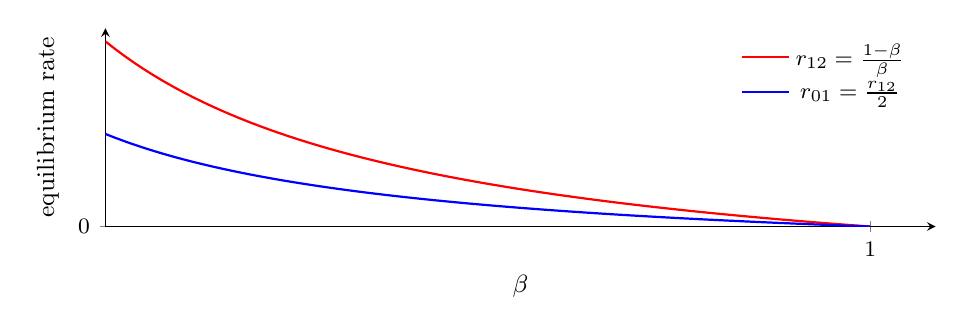
\begin{tikzpicture}
\begin{axis}[width=\linewidth,height=4.1cm,xmin=0.3,xmax=1.06,ymin=0,ymax=2.5,axis lines=left,xlabel={$\beta$},
  ylabel={equilibrium rate},xtick={1},xticklabels={$1$},ytick={0},yticklabels={$0$},
  legend style={font=\footnotesize,draw=none,fill=none,at={(0.98,0.98)},anchor=north east},
  label style={font=\small},tick label style={font=\footnotesize}]
\addplot[thick,red,domain=0.3:1,samples=80]{1/x-1};
\addplot[thick,blue,domain=0.3:1,samples=80]{(1-x)/(2*x)};
\legend{$r_{12}=\frac{1-\beta}{\beta}$,$r_{01}=\frac{r_{12}}{2}$}
\end{axis}
\end{tikzpicture}
\end{minipage}\hfill
\begin{minipage}[c]{0.5\linewidth}
\intuicao{Rates rise until each self is content with its endowment. Self 1 discounts date 2 by $\beta$, so $r_{12}=1/\beta-1$. Self 0
discounts date 1 by $\beta$ too, but values dates 1 and 2 equally, and a unit saved to date 1 is spread over both at the
high rate $r_{12}$: it needs only half the premium.}
\end{minipage}
\refbib{Kurlat (2020), ch.~9, \S9.1, eq.\ (9.1.8) (an endowment economy); Romer (2012), ch.~8, \S8.6.}
\rubrica{
\item Clearing and $r_{12}$ 1 pt; propensities and $r_{01}$ 1 pt. Rates from an Euler equation without clearing: max.\ half.
\item Graph, scored separately (1 pt): labelled axes; two decreasing curves vanishing at $\beta=1$; $r_{12}=2r_{01}$ above.
}
\end{sol}

\textbf{e)} (3 points) \emph{Parameter analysis.} Sign the effects of $\beta$, of $\sigma$ and of naivete (all households naive
instead of sophisticated, also in (d)) on $x$, $r_{01}$ and $r_{12}$; prove each sign and collect the signs in a table, give the
limits of $x$ at the ends of the admissible ranges, and read the results.
\resolespaco
\begin{sol}
\begin{center}
\begin{tabular}{lccc}
\toprule
Result & $\beta\uparrow$ & $\sigma\uparrow$ & naive instead of sophisticated \\
\midrule
$x$ (value of commitment) & $-$ near $\beta=1^{\dagger}$ & $-$ near $\beta=1^{\dagger}$ & perceived value $0$ \\
$r_{01}$ & $-$ & $0$ & sign of $\sigma-1$ \\
$r_{12}$ & $-$ & $0$ & $0$ \\
\bottomrule
\multicolumn{4}{l}{\footnotesize $^{\dagger}$Not monotone: $x\to0$ at both ends of each range.}
\end{tabular}
\end{center}
\passo{$x$ at the ends}{For $\sigma\ne1$, $1-x=B^{\eta}$ with $B\equiv\frac{1+\Lambda}{1+2\omega}$, $\eta\equiv\frac{\sigma}{1-\sigma}$. $\beta\to1$: $\omega\to1$, $\Lambda\to2$. $\beta\to0$: $\omega\to0$, $\Lambda\to0$
($\beta+\omega\to0$). $\sigma\to\infty$: $\omega\to1$, $\Lambda\to2$, $\eta\to-1$. $\sigma\to0$: $\omega\to0$, $\Lambda=\omega(1+\omega)^{1-1/\sigma}(1+\frac{\omega}{\beta})^{1/\sigma}\le\omega e^{\omega/(\beta\sigma)}\to0$, $\eta\to0$.
Each time $B\to1$ with $\eta$ bounded, so $x\to0$; under log too ($\beta\ln\beta\to0$ as $\beta\to0$).}
\passo{$x$: signs}{$x$ is continuous, positive inside and vanishes at both ends of each range, so it has an interior maximum
in $\beta$ and in $\sigma$: neither effect has a global sign. Near $\beta=1$, differentiating the smooth expansion of (c): $\partial_\beta x=-\frac{1-\beta}{6\sigma}+O((1-\beta)^2)<0$ and $\partial_\sigma x=-\frac{(1-\beta)^2}{12\sigma^2}+O((1-\beta)^3)<0$.}
\passo{rates}{$\partial_\beta r_{01}=-\frac1{2\beta^2}<0$, $\partial_\beta r_{12}=-\frac1{\beta^2}<0$, $\partial_\sigma r_{01}=\partial_\sigma r_{12}=0$; both vanish as $\beta\to1$ and diverge as $\beta\to0$.}
\passo{naive economy}{Self 1 is unchanged, so is $r_{12}$. A naive self 0 believes self 1 will maximize $u(c_1)+u(c_2)$ s.t.\ $c_1+\beta c_2=W_1$:
planned $c_1^p=\frac{W_1}{1+\beta^{p}}$, $p\equiv1-\frac1\sigma$, and by the envelope theorem $W_1$ is worth $\beta u'(c_1^p)$ at the margin. Its Euler
equation at $c_0=y$, $W_1=(1+\beta)y$ gives $1+r_{01}^N=\frac1\beta(\frac{1+\beta}{1+\beta^{p}})^{\sigma}$, which depends on $\sigma$. Against $1+r_{01}^S=\frac{1+\beta}{2\beta}$, taking
$1/\sigma$ powers: $r_{01}^N\gtreqless r_{01}^S\iff(\frac{1+\beta}2)^{p}\gtreqless\frac{1+\beta^{p}}2$. As $z^{p}$ is strictly concave for $p\in(0,1)$ ($\sigma>1$) and strictly
convex for $p<0$ ($\sigma<1$), $\operatorname{sign}(r_{01}^N-r_{01}^S)=\operatorname{sign}(\sigma-1)$. Knife-edge $\sigma=1$: naivete changes nothing but the perceived $x$.}
\intuicao{Commitment is worth most at intermediate present bias: it vanishes when the selves agree ($\beta\to1$, a
Harberger triangle), when self 0 ignores the future ($\beta\to0$), when self 1 splits evenly ($\sigma\to\infty$) and when every self
consumes at once ($\sigma\to0$). Sophisticates buy commitment; naifs, who lose more, do not: the case for defaults and
forced saving (401(k) defaults, Brazil's FGTS). Present bias raises real rates, $r_{12}=2r_{01}$, free of $\sigma$ under
sophistication; naivete moves $r_{01}$ only if $\sigma\ne1$.}
\refbib{Kurlat (2020), ch.~6, \S6.4 and ch.~9, \S9.1; Romer (2012), ch.~8, \S8.4 and \S8.6.}
\rubrica{
\item Signs proved, by row, the naive comparison included: 1.5 pts. Table: 0.5 pt. Limits of $x$: 0.5 pt. Reading: 0.5 pt.
\item Signs without proofs or reading: max.\ half. A limit or sign claimed without proof: 0 for that line.
}
\end{sol}
